\begin{adjustwidth*}{}{-2.25in}
\textbf{{\large Exercises}}
\setlength{\columnsep}{25pt}
\begin{multicols*}{2}
\noindent Terms and Concepts \small
\begin{enumerate}[1)]
\item T/F: The Product Rule states that $\ds \frac{d}{dx}\big(x^2\sin(x)\big) = 2x\cos(x)$.
\item T/F: The Quotient Rule states that $\ds \frac{d}{dx}\left(\frac{x^2}{\sin(x)}\right) = \frac{\cos(x)}{2x}$.
\item T/F: Regardless of the function, there is always exactly one right way of computing its derivative.
\end{enumerate} 

\noindent {\normalsize Problems} \small

\noindent {\bf In exercises 4--7, 
\ba
\item Use the Product Rule to differentiate the function.
\item Manipulate the function algebraically and differentiate without the Product Rule.
\item Show that the answers from (a) and (b) are equivalent.
\ea}

\begin{enumerate}[1),resume]
\item $\ds f(x) = x(x^2 + 3x)$
\item $\ds g(x) = 2x^2(5x^3)$
\item $\ds m(t) = (2t-1)(t+4)$
\item $\ds f(\theta) = (\theta^2 + 5)(3-\theta^3)$
\end{enumerate}

\noindent {\bf In exercises 8--12, 
\ba
\item Use the Quotient Rule to differentiate the function.
\item Manipulate the function algebraically and differentiate without the Quotient Rule.
\item Show that the answers from (a) and (b) are equivalent.
\ea}

\begin{enumerate}[1),resume]
\item $\ds f(x) = \frac{x^2 + 3}{x}$
\item $\ds g(x) = \frac{x^3 - 2x^2}{2x^2}$
\item $\ds h(s) = \frac{3}{4s^3}$
\item $\ds f(t) = \frac{t^2 - 1}{t + 1}$
\item $\ds f(x) = \frac{x^4 + 2x^3}{x + 2}$
\end{enumerate}

\noindent {\bf In exercises 13--26, differentiate the given function.}

\begin{enumerate}[1),resume]
\item $\ds f(x) = x \sin(x)$
\item $\ds f(t) = \frac{1}{t^2} (\csc(t) - 4)$
\item $\ds f(x) = \frac{x+7}{\sqrt{x}}$
\item $\ds g(x) = \frac{x^5}{\cos(x) - 2x^2}$
\item $\ds h(t) = \cot(t) - e^t$
\item $\ds h(x) = 7x^2 + 6x - 2$
\item $\ds f(x) = (16x^3 + 24x^2 + 3x) \frac{7x - 1}{16x^3 + 24x^2 + 3x}$
\item $\ds f(t) = \sqrt[5]{t} (\sec(t) + e^t)$
\item $\ds f(x) = \frac{\sin(x)}{\cos(x) + 3}$
\item $\ds g(x) = e^2 (\sin(\pi/4) - 1)$
\item $\ds g(t) = 4t^3 e^t - \sin(t) \cos(t)$
\item $\ds h(t) = \frac{2^t + 3}{3^t + 2}$
\item $\ds f(x) = x^2 e^x \tan(x)$
\item $\ds g(x) = 2x \sin(x) \sec(x)$
\end{enumerate}

\noindent {\bf In exercises 27--30, find the equation of the tangent line of the function at the given point.}

\begin{enumerate}[1),resume]
\item $\ds g(s) = e^s(s^2 + 2)$ at $(0,2)$
\item $\ds g(t) = t \sin(t)$ at $(3\pi/2, -3\pi/2)$
\item $\ds f(x) = \frac{x^2}{x-1}$ at $(2,4)$
\item $\ds f(t) = \frac{\cos(t) - 8t}{t + 1}$ at $(0,-5)$
\end{enumerate}

\noindent {\bf In exercises 31--34, find the $x$-values where the function has a horizontal tangent line.}

\begin{enumerate}[1),resume]
\item $\ds f(x) = 6x^2 - 18x - 24$
\item $\ds f(x) = x \sin(x)$ on $[-1,1]$
\item $\ds g(x) = \frac{x}{x+1}$
\item $\ds h(x) = \frac{x^2}{x+1}$
\end{enumerate}

\noindent {\bf In exercises 35--38, find the indicated derivative.}

\begin{enumerate}[1),resume]
\item $\ds f(x) = x \sin(x)$; find $f''(x)$
\item $\ds f(x) = x \sin(x)$; find $f^{(4)}(x)$
\item $\ds f(x) = \csc(x)$; find $f''(x)$
\item $\ds f(x) = (x^3 - 5x + 2)(x^2 + x - 7)$; find $f^{(8)}(x)$

\item Let $f$ and $g$ be differentiable functions for which the following information is known:  $f(2) = 5$, $g(2) = -3$, $f'(2) = -1/2$, $g'(2) = 2$.
\ba
	\item Let $h$ be the new function defined by the rule $h(x) = g(x) \cdot f(x)$.  Determine $h(2)$ and $h'(2)$.
	\item Find an equation for the tangent line to $y = h(x)$ at the point $(2,h(2))$.
	\item Let $r$ be the function defined by the rule $r(x) = \frac{g(x)}{f(x)}$.  Is $r$ increasing, decreasing, or neither at $a = 2$?  Why?
	\item Estimate the value of $r(2.06)$ by using the local linearization of $p$ at the point $(2,p(2))$.
\ea
\end{enumerate}

%------------------------------------------
% END OF EXERCISES ON FIRST PAGE
%------------------------------------------
\end{multicols*}
\end{adjustwidth*}

\clearpage

\begin{adjustwidth*}{}{-2.25in}
\setlength{\columnsep}{25pt}
\begin{multicols*}{2}\small

\begin{enumerate}[1),start=40]
\item Consider the functions $r(t) = t^t$ and $s(t) = \arccos(t)$, for which you are given the facts that $r'(t) = t^t(\ln(t) + 1)$ and $s'(t) = -\frac{1}{\sqrt{1-t^2}}$.  Do not be concerned with where these derivative formulas come from.  We restrict our interest in both functions to the domain $0 < t < 1$.
\ba
	\item Let $w(t) = t^t \arccos(t)$.  Determine $w'(t)$.
	\item Find an equation for the tangent line to $y = w(t)$ at the point $(\frac{1}{2}, w(\frac{1}{2}))$.
	\item Let $v(t) = \frac{t^t}{\arccos(t)}$.  Is $v$ increasing or decreasing at the instant $t = \frac{1}{2}$?  Why?
\ea

\item Let functions $p$ and $q$ be the piecewise linear functions given by their respective graphs below.  Use the graphs to answer the following questions.
\begin{center}
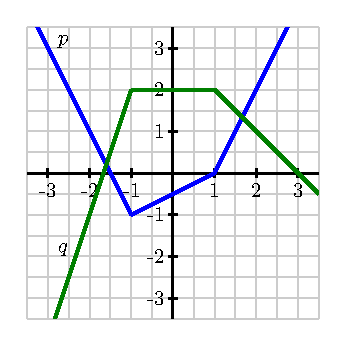
\includegraphics[scale=.75]{figures/2_1_Ez3.eps}
\end{center}
\ba
	\item Let $r(x) = p(x) \cdot q(x)$.  Determine $r'(-2)$ and $r'(0)$.
	\item Are there values of $x$ for which $r'(x)$ does not exist?  If so, which values, and why?
	\item Find an equation for the tangent line to $y = r(x)$ at the point $(2,r(2))$.
	\item Let $z(x) = \frac{q(x)}{p(x)}$.  Determine $z'(0)$ and $z'(2)$.
	\item Are there values of $x$ for which $z'(x)$ does not exist?  If so, which values, and why?	
\ea

\item A farmer with large land holdings has historically grown a wide variety of crops.  With the price of ethanol fuel rising, he decides that it would be prudent to devote more and more of his acreage to producing corn.  As he grows more and more corn, he learns efficiencies that increase his yield per acre.  In the present year, he used 7000 acres of his land to grow corn, and that land had an average yield of 170 bushels per acre.  At the current time, he plans to increase his number of acres devoted to growing corn at a rate of 600 acres/year, and he expects that right now his average yield is increasing at a rate of 8 bushels per acre per year.  Use this information to answer the following questions.
\ba
	\item Say that the present year is $t = 0$, that $A(t)$ denotes the number of acres the farmer devotes to growing corn in year $t$, $Y(t)$ represents the average yield in year $t$ (measured in bushels per acre), and $C(t)$ is the total number of bushels of corn the farmer produces.  What is the formula for $C(t)$ in terms of $A(t)$ and $Y(t)$?  Why?
	\item What is the value of $C(0)$?  What does it measure?
	\item Write an expression for $C'(t)$ in terms of $A(t)$, $A'(t)$, $Y(t)$, and $Y'(t)$.  Explain your thinking.
	\item What is the value of $C'(0)$?  What does it measure?
	\item Based on the given information and your work above, estimate the value of $C(1)$.	
\ea

\item Let $f(v)$ be the gas consumption (in liters/km) of a car going at velocity $v$ (in km/hour). In other words, $f(v)$ tells you how many liters of gas the car uses to go one  kilometer if it is traveling at $v$ kilometers per hour. In addition, suppose that $f(80)=0.05$ and $f'(80) = 0.0004$.
\ba
	\item Let $g(v)$ be the distance the same car goes on one liter of gas at velocity $v$.  What is the relationship between $f(v)$ and $g(v)$? Hence find $g(80)$ and $g'(80)$.
      	\item Let $h(v)$ be the gas consumption in liters per hour of a car going at velocity $v$. In other words, $h(v)$ tells you how many liters of gas the car uses in one hour if it is going at velocity $v$.   What is the algebraic relationship between $h(v)$ and $f(v)$?  Hence find $h(80)$ and $h'(80)$.     
	\item How would you explain the practical meaning of these function and derivative values to a driver who knows no calculus?  Include units on each of the function and derivative values you discuss in your response.  
\ea

\item An object moving vertically has its height at time $t$ (measured in feet, with time in seconds) given by the function $h(t) = 3 + \frac{2\cos(t)}{1.2^t}$.
\ba
	\item What is the object's instantaneous velocity when $t =2$?
	\item What is the object's acceleration at the instant $t = 2$?
	\item Describe in everyday language the behavior of the object at the instant $t = 2$.
\ea

\item Let $f(x) = \sin(x) \cot(x)$.
\ba
	\item Use the product rule to find $f'(x)$.
	\item True or false: for all real numbers $x$, $f(x) = \cos(x)$.
	\item Explain why the function that you found in (a) is almost the opposite of the sine function, but not quite.  (Hint: convert all of the trigonometric functions in (a) to sines and cosines, and work to simplify.  Think carefully about the domain of $f$ and the domain of $f'$.)
\ea
\end{enumerate}

%---------------------------------------------
% END OF EXERCISES ON SECOND PAGE
%---------------------------------------------
\end{multicols*}
\end{adjustwidth*}

\afterexercises